%%% TeX-master: "manuscript"
% !TeX spellcheck=en_GB

\newpage

\section{Figure Legends}

\subsection{Figure 1}

\begin{figure}[ht]
  \centering
  \includegraphics{fig_1_pathway_overview}
  \caption{\textbf{Schematic overview of NAD biosynthesis and consumption.} NAD can be synthesised from tryptophan (Trp), nicotinamide (Nam), nicotinic acid (NA), and, to a lesser extend, nicotinamide ribose (NR). Nam is the main precursor and also the product of NAD-consuming signalling reactions by enzymes such as sirtuins (NAD-dependent histone deacetylases) or PARPs (poly-ADP-ribosylases). For the recycling of Nam, two different pathways exist. The pathway found in yeast and many bacteria starts with the deamination of Nam by Nam deamidase (NADA). The other three enzymes comprise the Preiss-Handler pathway that also exists in vertebrates. The pathway found in vertebrates directly converts Nam into the corresponding mononucleotide (NMN) by the Nam phosphoribosyltransferase (NamPRT). A third enzyme can consume Nam, the Nam N-methyltransferase (NNMT). For more details and abbreviations, see text.}
  \label{fig:pathway_overview}
\end{figure}

\newpage


\subsection{Figure 2}

\begin{figure}[ht]
  \centering
  \includegraphics[width=0.75\textwidth]{fig_2_phylo_distribution}
  \caption{\textbf{Evolutionary distribution of NADA, NNMT and NamPRT and their relation to the number of NAD consumers.} A) Distribution of NADA, NNMT and NamPRT in selected major taxa. NADA is dominant in Bacteria, Fungi, and Plants (Viridiplantae), whereas NamPRT together with NNMT is dominant in Metazoa. Numbers at the pie charts show, how many species of the taxon possess the respective enzyme combination indicated by the colour explained in the lower right of the figure. Below the taxon name, the number of species in that taxon is given. B) Common tree of selected taxa within the Metazoa, including 334 species. The pie charts indicate the distribution of species within the respective taxon that have the enzyme combination indicated by the colour explained in the lower right. The size of the pie charts is proportional to the logarithm of the number of species analysed in the particular taxon. The numbers below the taxon names indicate the average number of NAD-consuming enzyme families found in all sub-taxa. The branch length is arbitrary.}
  \label{fig:phylo_distribution}
\end{figure}

\newpage


\subsection{Figure 3}

\begin{figure}[ht]
  \centering
  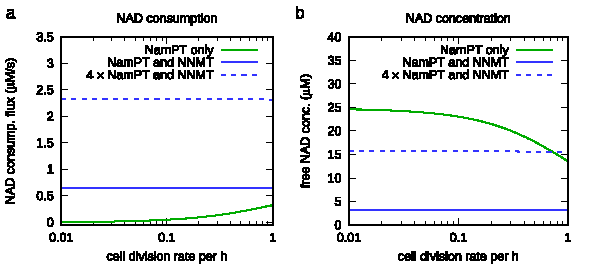
\includegraphics[width=\textwidth]{fig_3_NNMT_NAD_flux}
  \caption{\textbf{NNMT enables high NAD consumption flux.} We used a dynamic model of NAD biosynthesis and consumption (details see Materials and Methods) to simulate NAD consumption flux (A) and NAD concentration (B) in the presence of NamPRT and with or without NNMT at different cell division rates. NNMT enables higher steady state NAD consumption flux despite reduced NAD concentrations.}
  \label{fig:NNMT_NAD_flux}
\end{figure}

\newpage


\subsection{Figure 4}

\begin{figure}[ht]
  \centering
  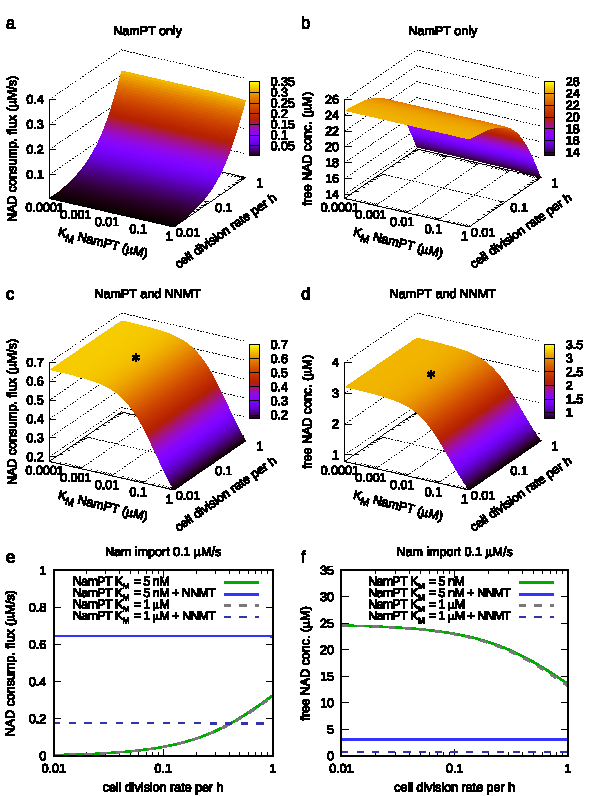
\includegraphics[width=0.9\textwidth]{fig_4_NamPRT_affinity_Nam}
  \caption{\textbf{Role of NamPRT affinity for Nam.} Using the dynamic model of NAD biosynthesis and consumption we simulated the affect of different Michaelis-Menten constants ($K_M$) of NamPRT for Nam on steady state NAD consumption flux and NAD concentration at different cell division rates. In the absence of NNMT (A and B), the $K_M$ of NamPRT has little influence on NAD consumption and concentration, but both are changing with cell division rates. In the presence of NNMT (C and D), decreasing $K_M$ of NamPRT enables increasing NAD consumption flux and NAD concentration. NNMT furthermore makes both, consumption flux and concentration, relatively independent of cell division rates. Comparing the situation with and without NNMT (E and F) at different NamPRT $K_M$ reveals that at low $K_M$ and high cell division rates NNMT no longer enables higher NAD consumption rates compared to NamPRT alone.}
  \label{fig:NamPRT_affinity_Nam}
\end{figure}

\newpage


\subsection{Figure 5}

\begin{figure}[ht]
  \centering
  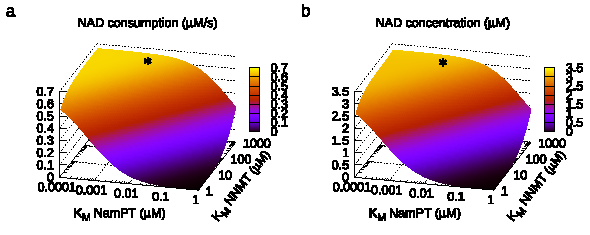
\includegraphics[width=\textwidth]{fig_5_optimal_substr_affinities}
  \caption{\textbf{The substrate affinities of human NNMT and NamPRT are optimal.} Both NAD consumption flux (A) and NAD concentration (B) are increasing with decreasing $K_M$ of NamPRT but decreasing $K_M$ of NNMT. The affinities reported for human enzymes (indicated by a black asterisk) appear to be close to optimal, as further improvements would have little or no effect on NAD consumption or concentration.}
  \label{fig:optimal_substr_affinities}
\end{figure}

\newpage


\subsection{Figure 6}

\begin{figure}[ht]
  \centering
  \includegraphics[width=0.75\textwidth]{fig_6_unresolved_loop}
  \caption{\textbf{The function of the structurally unresolved loop structure of NamPRT.} Most Deuterostomia that encode NNMT show a sequence insertion in the N-terminal region of NamPRT that has been revealed by multiple sequence alignment of NamPRT from different species (A). Coloured circles indicate the enzymes present in the species besides NamPRT; blue: NNMT; black: NADA and NNMT; yellow: NADA. For a more comprehensive alignment, please see supplementary figure~S1. B) The visualisation of human NamPRT is based on a structure prediction of SWISS-MODEL \cite{Arnold2006,Biasini2014} of the sequence of the human NamPRT using the model 2H3D as template \cite{Wang2006}. The inserted region is not resolved in crystal structures of NamPRT and thus appears to be a flexible loop structure at the surface of the NamPRT dimer, coloured in red. C) The localisation of the FLAG-tagged mutant protein lacking the unresolved loop is not changed compared to wildtype human NamPRT. Both show a heterogeneous nuclear cytosolic localisation in immunofluorescence images in HeLa S3 cells. But \textit{in vitro} measurements using recombinant protein show that the mutant NamPRT has lower activity than the wildtype enzyme (D) and is not activated by ATP (E). Bars in D) and E) with different letters indicate significant difference as estimated with a T test assuming independent samples and significance at $p < 0.05$.}
  \label{fig:unresolved_loop}
\end{figure}

\newpage


\subsection{Figure 7}

\begin{figure}[ht]
  \centering
  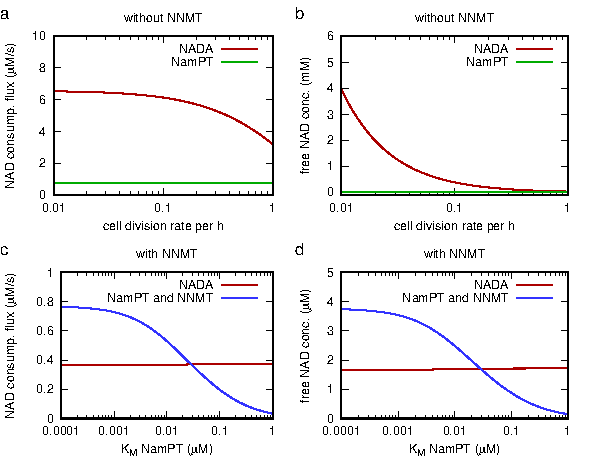
\includegraphics[width=\textwidth]{fig_7_NNMT_comp_advantage}
  \caption{\textbf{NNMT provides a competitive advantage and makes NADA obsolete.} To simulate competition for common resources, we created a two compartment model where one compartment contained NADA but no NamPRT and the other compartment contained NamPRT either with or without NNMT but no NADA. In the absence of NNMT (A and B) the compartment containing NADA has slightly lower NAD consumption rates (A) but much higher NAD concentrations (B). In the presence of NNMT, however, both NAD consumption (C) and NAD concentration (D) are lower in the NADA compartment, but this effect is only observed at low NamPRT $K_M$.}
  \label{fig:NNMT_comp_advantage}
\end{figure}

\newpage


\subsection{Figure 8}

\begin{figure}[ht]
  \centering
  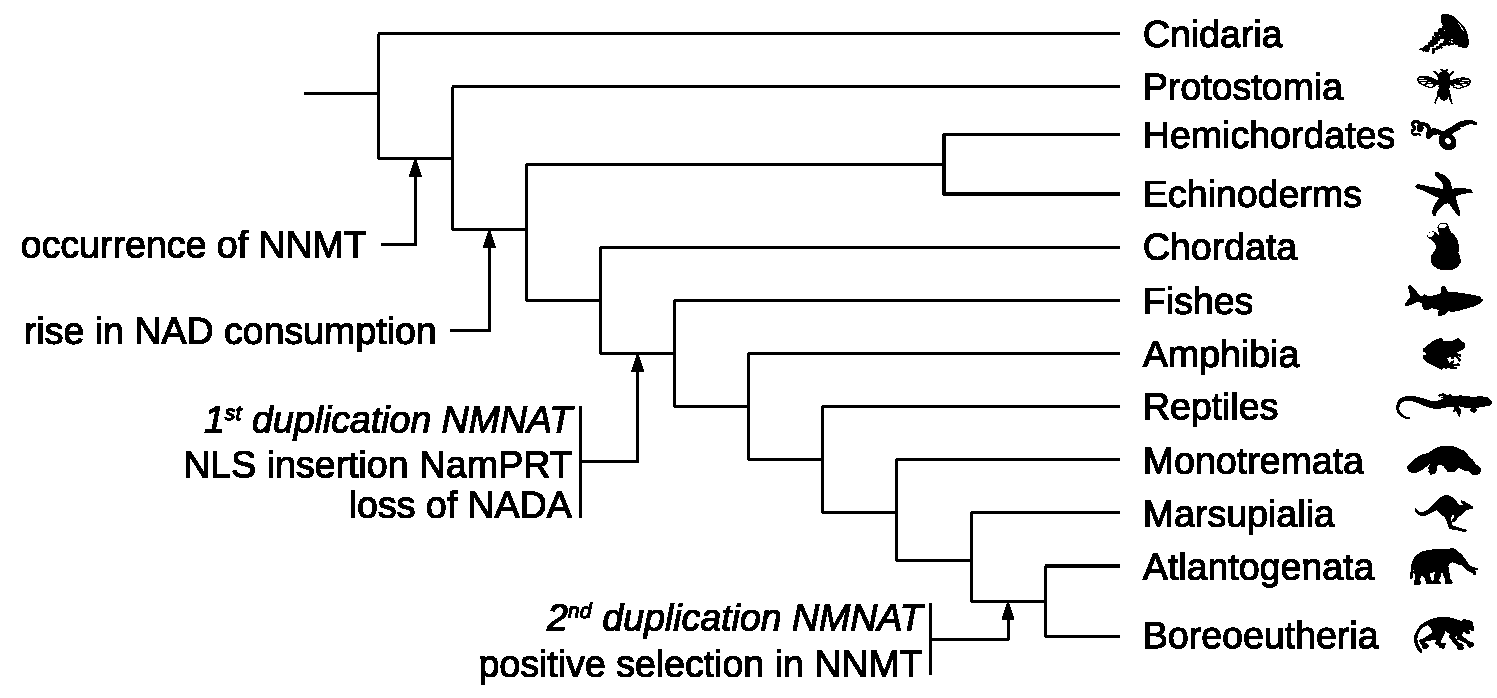
\includegraphics[width=\textwidth]{fig_8_evo_events}
  \caption{\textbf{Loss of NADA is accompanied by NamPRT loop insertion.} We indicated important events in NAD salvage pathways in this phylogenetic tree of Metazoa. Duplications of NMNAT according to \cite{Lau2010}. \todo{What about the positive selection in NNMT?}}
  \label{fig:evo_events}
\end{figure}

\newpage
